\documentclass[twoside,onecolumn,fleqn,a4paper,12pt]{prop-spsitb}
%
\usepackage{graphicx}
\usepackage{color, openbib, rotate, amsfonts, amsmath, amssymb}
\usepackage[left=4cm, right=3cm, top=3cm, bottom=3cm]{geometry}

%\usepackage[colorlinks,linkcolor=black,urlcolor=black]{hyperref}
\setcounter{tocdepth}{2}
\usepackage[bookmarksopen=true,bookmarks=true]{hyperref}
\usepackage{bookmark}

\usepackage{url}
\usepackage{float}
  \floatplacement{figure}{H}
  \floatplacement{table}{H}
%\usepackage{multirow}
\usepackage{makeidx}
\usepackage[mathcal]{euscript}
\usepackage[bahasa]{babel}
\usepackage{listings}
\usepackage{color}

%\usepackage{lscape}
\usepackage{pdflscape}
\usepackage{titlesec}

\usepackage{natbib}
\bibliographystyle{apa-good}
\setlength{\bibhang}{1.2cm}

%\titleformat{\chapter}[display]
%{\normalfont\huge\bfseries\centering}{\chaptertitlename\ \thechapter}{20pt}{\Huge}

\definecolor{dkgreen}{rgb}{0,0.6,0}
\definecolor{gray}{rgb}{0.5,0.5,0.5}
\definecolor{mauve}{rgb}{0.58,0,0.82}

\newcommand{\pic}{Figure}
\newcommand{\tab}{Table}
\newcommand{\equ}{Equation}

\renewcommand\thechapter{\Roman{chapter}}

\setcounter{secnumdepth}{3}

\usepackage{xcolor}
\hypersetup{
    colorlinks,
    linkcolor={black},
    citecolor={black},
    urlcolor={black}
}

\hyphenation{
	con-si-der-ing
	e-mi-ssion
	ca-li-bra-tion
	self-ca-li-bra-tion
	pa-ra-meter
	pa-ra-meters
}

\usepackage[onehalfspacing]{setspace}

% Menghilangkan indentasi paragraf
\setlength{\parindent}{0pt}

% Menghilangkan semua spasi sebelum dan setelah section/subsection
\titlespacing*{\section}{0pt}{0pt}{0pt}
\titlespacing*{\subsection}{0pt}{0pt}{0pt}

\newcommand{\resetparskip}{\setlength{\parskip}{0em}}
\newcommand{\restoreparskip}{\setlength{\parskip}{1em}}
%
\begin{document}
%
\frontmatter
\pagestyle{empty}
\begin{titlepage}
\begin{center}
\mbox{}
\vspace{1cm}

\textbf{CONTINUUM DEEP-FIELD DETECTION AND \\ ANALYSIS IN SUB-MM AROUND RADIO GALAXIES: \\ DUST AND SYNCHROTRON EMISSIONS}

\vspace{3cm}

\textbf{DOCTORAL RESEARCH PROPOSAL}\\

\vspace{3cm}

\normalsize{By}

\textbf{Nama Mahasiswa}

\textbf{NIM: 081320}

\textbf{(Doctoral Study Program of Astronomy)}

\vspace{2.0cm}

\begin{figure}[!h]
\centering

\includegraphics[width=2.35cm, height=3.5cm]{fig/logo_itb.png}
\end{figure}

\vspace{2.0cm}

\textbf{INSTITUT TEKNOLOGI BANDUNG}

\textbf{April 2025}

\end{center}
\end{titlepage}

\cleardoublepage
%\thispagestyle{empty}


\newpage
\begin{center}
\textbf{ABSTRAK}

\vspace{0.5cm}

\textbf{DETEKSI DAN ANALISIS EMISI DEBU DAN SINKROTRON DI LINGKUNGAN GALAKSI RADIO MELALUI 
CITRA KONTINUM \textit{DEEP-FIELD} DALAM RENTANG SUBMILIMETER DARI PENGAMATAN ALMA}\\
\vspace{0.5cm}

Oleh\\
\textbf{Nama Mahasiswa\\
NIM: 081320\\
Program Studi Doktor Astronomi}\\
\end{center}

\vspace{1.0cm}
\restoreparskip
Galaksi radio merupakan salah satu jenis {\it galaksi aktif} yang memancarkan energi sangat kuat pada panjang gelombang radio, dengan daya dalam rentang $10^{34}$ -- $10^{39}$ W. Pada umumnya mereka merupakan galaksi elips yang sangat masif, yang masih mengandung materi antar bintang dingin dan rapat. Keberadaan debu di galaksi radio dideteksi dari emisi inframerah-jauh (\textit{far-infrared}, FIR). Hal ini diduga dapat berasal dari proses pemanasan oleh bintang muda masif ataupun dari \textit{active galactic nuclei} (AGN). Berbagai mekanisme telah diusulkan untuk menjelaskan asal usul emisi tersebut, namun kontribusi dari masing-masing mekanisme masih belum dapat dipastikan.

Radio-AGN kuat biasanya mengandung sedikit gas molekuler dengan massa rata-rata sekitar $10^8$ M$_\odot$ pada galaksi induknya. Gas tersebut biasanya dideteksi sebagai pasokan ke cakram akresi yang mengelilingi inti, berupa lubang hitam sangat masif (SMBH), yang menghasilkan berbagai aktivitas inti. Dari beberapa penelitian lain, galaksi-galaksi tipe-awal tidak menunjukkan laju pembentukan bintang yang cepat, sehingga memberikan dugaan bahwa baik bintang-bintang tua ataupun AGN dapat menjadi sumber dari emisi FIR tersebut. Selain itu terdapat indikasi bahwa kandungan gas di galaksi elips tidak terkait dengan populasi bintang dan lebih menganjurkan pasokan gas yang berasal dari luar galaksi. Mekanisme yang membawa gas molekular ke daerah pusat diduga adalah proses \textit{merger} galaksi. Terdapat tiga jenis \textit{merger} berdasarkan kandungan gas yang dibawa, yaitu \textit{merger} basah (\textit{merger} antara dua galaksi kaya gas), kering, dan campuran.  Aktivitas galaksi radio bertipe Fanaroff-Riley I (FR I) diduga dipicu oleh akresi kering (\textit{Bondi accretion}), sedangkan tipe FR II dipicu oleh banyaknya pasokan gas yang masuk ke daerah pusat melalui proses \textit{minor-merger} basah.

Galaksi radio yang biasanya bertepatan dengan galaksi elips di optik, umumnya berada di tengah kumpulan galaksi yang cukup rapat, sehingga mempelajari sifat-sifat materi antar bintang (ISM) dari galaksi-galaksi di sekitar galaksi radio ini menjadi sangat penting guna memahami proses pembentukan galaksi radio, evolusi, serta umpan baliknya terhadap lingkungan. Untuk itu, dalam disertasi ini, kami mengusulkan untuk melakukan  studi terperinci lingkungan galaksi radio yang diamati oleh {\it Atacama Large Millimeter/submillimeter Array} (ALMA), yang sejauh ini merupakan teleskop radio paling sensitif dalam rentang panjang gelombang submilimeter. Data yang diperoleh dari pengamatan kalibrator untuk setiap proyek sains ALMA, yang sebagian besar merupakan galaksi radio, akan dianalisis secara terperinci. Setelah melalui proses seleksi terhadap target yang tepat dan dengan menggabungkan sejumlah data yang terkumpul, citra  kontinum submilimeter dengan tingkat derau yang sangat rendah ({\it deep-field submm images}) dalam orde puluhan $\mu$Jy haruslah dapat diperoleh. Dengan data tersebut emisi termal dan/atau sinkroton di bagian pusat galaksi haruslah dapat ditentukan. Demikian pula pengaruh distribusi ISM terhadap daerah pusat AGN beserta lingkungannya akan dapat dipelajari. Analisis selanjutnya akan dapat membantu membedakan sumber pemanasanan debu, apakah berasal dari pembentukan bintang ataukah dari AGN.

\vspace{1em}

\noindent Kata kunci: AGN, galaksi radio, kalibrator, kontinum, submilimeter
\resetparskip





\addcontentsline{toc}{chapter}{ABSTRAK}

\newpage
\begin{center}
\textbf{ABSTRACT}

\vspace{0.5cm}

\textbf{CONTINUUM DEEP-FIELD DETECTION AND \\ ANALYSIS IN SUB-MM AROUND RADIO GALAXIES: \\ DUST AND SYNCHROTRON EMISSION}\\
\vspace{0.5cm}

By\\
\textbf{Nama Mahasiswa\\
NIM: 081320\\
Doctoral Study Program of Astronomy}\\
\end{center}

\vspace{1.0cm}
\restoreparskip
Radio galaxies constitute a type of \textit{active galaxies} that generate enormous radio power in the range of $10^{34}$ -- $10^{39}$ W. Most of them are hosted by  massive elliptical galaxies which still contain some dense and cold interstellar medium (ISM). Dust emission is mainly detected in the far-infrared (FIR) radiation which is assumed to be thermal and originated from heating processes either by young massive stars or by the active galactic nuclei (AGN). Different mechanisms were proposed to explain the originof these emissions but their respective contributions are not yet conclusive.

Powerful radio-AGN are usually very poor in molecular gas with an average mass of a few $10^8$ M$_\odot$ in the host galaxy. The gas is usually detected as a circumnuclear disk necessary to feed the accretion disk around the central supermassive black hole (SMBH), generating the nuclear activity. In contrast, early-type galaxies -- correspond to elliptical galaxies -- have shown no independent evidence of high star formation rates (SFRs), suggesting that either the older stars or the AGN are responsible for much of the FIR emission. One also argued that in  elliptical galaxies the gas is unrelated to the stellar populations and favor an external origin of the molecular gas. Furthermore, it has been argued that Fanaroff-Riley Type I (FR I) radio galaxies are triggered through a ``dry'' accretion while those of FR II radio galaxies by molecular gas fed towards the center. It has been suggested that ``wet''  minor mergers would be a mechanism to bring molecular gas and dust towards the center which triggers the radio activity.

The radio galaxies (hosted by elliptical galaxies) are frequently found in dense concentration of galaxies, and thus it is crucial to study the ISM properties of the galaxies around these radio galaxies to be able to understand the formation, evolution, and the feedback of the radio galaxy to their environment. To do so, in this dissertation work, we propose to undertake detailed studies in the field of radio galaxies observed by the Atacama Large Millimeter/submillimeter Array (ALMA), which offers unprecedented sensitivity, to investigate particularly the environment around radio galaxies. We will exploit the data acquired from the calibration observations performed for each science project of ALMA. Calibrations are always made, by observing known radio sources that are in vast majority radio galaxies, to set various observational parameters. After selecting some appropriate targets, and by combining the accumulated compatible data, we should be able to reach a sufficiently low noise level at tens $\mu$Jy to obtain deep submillimeter images. We will measure the thermal and/or synchrotron emission in the central radio galaxy and in the field to study the distribution of the ISM and the interplay between the central AGN and its environment. Further analyses should also permit us to disentangle the source of dust heating, AGN or star formation.

\vspace{1em}

\noindent Key words: AGN, radio galaxies, calibrators, continuum, submillimeter

\resetparskip




\addcontentsline{toc}{chapter}{ABSTRACT}

\newpage
%\pagestyle{empty}
\begin{center}
{\normalsize \textbf{CONTINUUM DEEP-FIELD DETECTION AND \\ ANALYSIS IN SUB-MM AROUND RADIO GALAXIES: \\ DUST AND SYNCHROTRON EMISSION}\par}
\vskip 1.2cm

{\normalsize By}\\
{\normalsize \textbf{Mahasiswa\\
NIM: 081320\\
Doctoral Study Program of Astronomy}\par}

%\vskip 2cm

{\normalsize Institut Teknologi Bandung} \\

\vskip 2cm

Approved by \\
Supervisor Team \par

\vskip 0.5cm

Date: 9 April 2018 \par

\vskip 1.0cm

Chair\par

\vskip 2.0cm

\rule{4.5cm}{0.4pt}\\[.5ex]
Prof. Dr. A

\vskip1.0cm

\begin{tabular}{ccc} %{\textwidth}{cXc}
Member &\hspace{4cm} & Member\\
%\includegraphics[scale=0.15]{fig/sleon_sign.png} & \\
\rule{4.5cm}{0.4pt} &\hspace{4cm} & \rule{4.5cm}{0.4pt}\\[.5ex]
Dr. B &\hspace{4cm} &  Dr. C 
\end{tabular} 



\end{center}


\cleardoublepage


\addcontentsline{toc}{chapter}{LEMBAR PENGESAHAN}

\newpage
\begin{center}
\textbf{PREFACE}
\end{center}

\vspace{0.5cm}

\textit{Alhamdulillah}, I would like to thank to Allah SWT, who gives me kindness and grace so I can live, to start 
this research, and also to finish this doctoral research proposal.

This doctoral research proposal can be completed with the support from people around me. I really would like to thank to:
\begin{itemize}
\item My family, my wife and my son who always give me the motivation to pursue this career.
\item Prof. , Dr. , Dr. , and Dr. , as my supervisors 
and mentors. Their valuable insights and directions gave me needful guidance to build this proposal and complete the research.
\item All my friends and students who always support me and give me inspiration. 
\end{itemize}

Any suggestion and correction to improve this doctoral research proposal would be greatly appreciated. 
Therefore, I would be very happy to hear any comment.

\vspace{2cm}
\begin{flushright}
Bandung, 22 Januari 2018

\vspace{1cm}

Nama Mahasiswa
\end{flushright}
\addcontentsline{toc}{chapter}{KATA PENGANTAR}

\tableofcontents
\addcontentsline{toc}{chapter}{DAFTAR ISI}

\listoffigures
\addcontentsline{toc}{chapter}{DAFTAR GAMBAR}

\listoftables
\addcontentsline{toc}{chapter}{DAFTAR TABEL}

\newpage
\begin{center}
    \textbf{\large DAFTAR SINGKATAN DAN LAMBANG}
\end{center}
    
\vspace{0.5cm}

\begin{table}[!ht]
    \centering
        \begin{tabular}{|c|c|c|}
            \hline
            Singkatan   & Nama & Halaman \\
            \hline
            AMR & \raggedright Adaptive Mesh Refinement & 1 \\
            \hline
            CT & \raggedright Computed Tomography & 2 \\
            \hline
            HPLC & \raggedright High Performance Liquid Chromatography & 5 \\
            \hline
        \end{tabular}
\end{table}

\begin{table}[!ht]
    \centering
        \begin{tabular}{|l|l|c|}
            \hline
            \multicolumn{1}{|c|}{Lambang} & \multicolumn{1}{c|}{Nama} & \multicolumn{1}{c|}{Halaman} \\
            \hline
            Data 1 & High Performance Liquid Chromatography & 1 \\
            \hline
            Data 2 & High Performance Liquid Chromatography  & 2 \\
            \hline
            Data 3 & High Performance Liquid Chromatography  & 3 \\
            \hline
        \end{tabular}
\end{table}



    
    
    
    
\addcontentsline{toc}{chapter}{DAFTAR SIMBOL DAN LAMBANG}

% mulai penomeran arabic
\pagestyle{plain}
\mainmatter
\chapter{Introduction}
\pagenumbering{arabic}

\section{Background}
Radio galaxies are a type of active galaxies that emit enormous radio luminosities, in the range of $10^{41}$ to $10^{46}$ erg s$^{-1}$ or equivalent to $10^{34}-10^{39}$ watts. They are one of the types of radio-loud active galaxy together with radio-loud quasar and blazar \citep{miley2008}. However, in this work, we use the  term ``radio galaxy'' for all types of radio-loud active galaxy. These objects can be detected at large distances, making them valuable tools for observational cosmology and the study of galaxy evolution.

Radio galaxies are divided mainly in two groups, the Fanaroff and Riley type I (FR-I) and type II (FR-II). As explained by \cite{fanaroff1974}, the sources were classified using the ratio of the distance between the regions of highest brightness of the radio continuum on opposite sides of the central galaxy or quasar, to the total extent of the source measured from the lowest contour; those sources from which the ratio was less than 0.5 were placed in class I, and those from which the ratio was greater than 0.5 were placed in class II. There is also a third classification called FR-c galaxies, covering galaxies that have a very compact radio continuum emission. Their radio morphologies suggest that they are compact versions of the classical FR-II's, although why they are so small is not yet established. It is hypothesized that these are either young FR-II's or FR-II's trapped in a dense environment \citep[e.g.][]{fanti1990, odea1991, fanti1994}.

The origin of the radio emission was studied in the last decade and still the complete picture about the physical processes are under debate \citep[e.g.][]{sikora1997, merloni2007, moderski1998}. In general, there are three types of merger of galaxy based on gas richness, wet (i.e. a merger between gas-rich galaxies), dry, and mixed merger. Based on the size of the galaxy, there are minor merger, when one of the galaxies is significantly larger than the other(s), and major merger, when two spiral galaxies that are approximately the same size collide. It has been argued that FR II radio galaxies, are triggered by molecular gas fed towards the center \citep{buttiglione2010} while the FR I type are triggered through a dry accretion (Bondi accretion) in the Broad Line Region \citep[BLR, see][]{fromerth2001}. It has been suggested that ``wet'' minor mergers would be a mechanism to bring molecular gas and dust towards the center of the radio galaxies and trigger the radio activity \citep[see, for example,][]{lim2000, israel1998}. A key aspect is the ability to feed the accretion disk around the central Supermassive Black Hole \citep[SMBH, see][]{merloni2008}.
 
The location of radio galaxies are normally overlap with giant elliptical galaxies with visual luminosities of about 2.1$\times$10$^{10} h^{-2}$ L$_\odot$  \citep{kellerman1988}. Although elliptical galaxies in general are relatively deficient in cold or molecular gas, observations of CO(J = 1$\rightarrow$ 0) emission lines indicate they still contain some dense and cold Interstellar Medium (ISM) \citep[e.g.,][]{wiklind1986}. Dust is also detected in those galaxies from the far-infrared (FIR) radiation. The radiation is assumed to be thermal and to originate from dust heated by either young massive stars or by the active galactic nuclei (AGN). According to \cite{kennicutt1998}, early-type galaxies -- correspond to elliptical galaxies -- show no independent evidence of high star formation rates (SFRs), suggesting either the older stars or the AGN are responsible for much of the FIR emission. \cite{wiklind1995} show that in elliptical galaxies, the gas is unrelated to the stellar populations, and favor an external origin of the molecular gas. 

It is then important to study the environment of radio galaxies and the ISM properties of the interstellar medium of the neighbor galaxies \citep{miley2008} to be able to understand the formation, the evolution and the feedback of the radio galaxy to their environment.  Measuring the molecular gas content in all the satellites would be, by far, too time consuming. However, the detection of the dust, a very good proxy of the global ISM, in a deep submm image would give valuable information on the amount of ISM  together with the star formation and/or possible activity in the neighbor galaxies. Moreover, it is possible to use only the radio  continuum emission since the molecular gas and dust are tightly linked by the correlation between IR luminosity as a tracer of dust, and HCN luminosity as a tracer of molecular gas in e.g. \cite{omont1996} and \cite{gaosolomon2004}. Such a detailed study is possible thanks to the advent of the Atacama Large Millimeter/submillimeter Array (ALMA), the largest radio interferometer array in the world, located in Northern Chile. Therefore, in this dissertation work, we propose to undertake a detailed study of the radio galaxy environments by using large amount of calibrator data provided by ALMA, available since the past few years. Detailed of the work will be described hereafter. 

\section{Objectives}

The objectives of this doctoral work will be:

\begin{enumerate}
\item To build a very deep catalogue of the dust emission in and around radio galaxies. This objective can be achieved by studying several radio galaxies covering a large redshift range from 0 to 2 with a very deep sensitivity on the order of a few tens of $\mu$Jy by using ALMA's calibrator data and obtaining the deepest image so far in continuum for the ALMA observing bands available at the time of this dissertation work (most likely in bands 3, 4, 6, 7, 8 and possibly 9), in the range of frequency from 84 GHz to 720 GHz.  

\item To uncover the physical origin of the radio continuum emission as being either thermal or synchrotron by building the Spectral Emission Distribution (SED) using the different ALMA bands. Once the discrimination is done, the main physical properties (dust mass, dust temperature, radio jet spectral index, etc) can be derived.

\item By using the built catalogue, we want to analyze the environment effects on the ISM content in these objects together with the effect of the galaxy evolution through the cosmic time (redshift). In particular, the dust content will be studied in the dense galaxy clusters hosting  the radio galaxies.

\item To analyze the synchrotron emission (radio jets) with the high angular resolution, in particular its interaction with the dust in the host elliptical galaxies and also in the environment.
\end{enumerate}

An in-depth analysis for individual radio galaxies will be performed depending on the features found in the corresponding deep sub-millimeter images. In addition, a sub-product of the work is a complete catalogue of the several absorption lines probably detected towards the strong radio continuum emission of these quasars.  These absorption lines presumably originate from our own Galaxy. Therefore, these data may be used to retrieve a map of molecular cloud in our Galaxy.

\section{Scope}
Scope of this project includes:

\subsection*{Data}
ALMA has been in operation since the end of 2011 by the Cycle 0 (Early Science Programs), conducted using 15 -- 20 antennas available at this period. Subsequently, the Cycle 1 was performed starting at the end of 2012, using many more antennas (more than 30), and so on. Presently, ALMA has been conducting the Cycle 5 for scientific community with more than 40 antennas. Accordingly, from then on, large data are available in public domain, since ALMA applied a short term proprietary period of one year only. Hence, all science projects will be available in public domain within one year after being delivered to the principal investigator. Correspondingly, for each science project, observations of different calibrators were performed (mainly radio galaxies or solar system objects) to derive a correct amplitude, phase and the frequency response of the ALMA correlators.

This research is aimed to produce a very deep (sensitivity in the order of a few tens of $\mu$Jy) catalogue of the dust emission in and around radio galaxies. However, the scope of our investigation will be limited to data from Cycle 1, 2, 3, and partly 4. Cycle 0 will not be explored since at the time, only a few number of antennas were used to collect the data, offering low sensitivity images which will not be significantly change the result if added to the more recent cycles data. Data from Cycle 5 is not publicly available yet, therefore can not be utilized for our project. We will  only select calibrators which have observational data at least from band 3, 6, and 7, to build the SED.

\subsection*{Cooperation}
This doctoral research work is a part of cooperation between Department of Astronomy, Faculty of Mathematics and Natural Sciences -- ITB and the European Southern Observatory (ESO) Part of the Joint ALMA Observatory (JAO), Santiago, Chile. Therefore, it is expected that some parts of this work will be conducted in Chile. 


\section{Method}

We note that every ALMA science project always includes calibration observations of very bright, compact sources to determine the flux density scale, to specify the bandpass response, and finally to calibrate the amplitude and phase of the visibilities  of the science targets. Most of bright radio sources are radio galaxies. Therefore, survey of these galaxies can be performed by analysing the data provided from calibration observations.

To achieve this goal, since the data are very big, we need to develop a pipeline that include maximizing the automatization of the data reduction. This includes the downloading, (self-)calibration, concatenation, as well as image ``cleaning''/filtering.  The final images will be denoised by applying a wavelet filtering 
\citep[e.g.,][]{leon2000} to improve the S/N.

After defining several criteria for selecting the calibrator samples, we should be able to study numerous radio galaxies in the range of  redshift from 0 to 2 (note that $z = 2$ corresponds to the age of the universe of about $\sim 3.3$ Gyr, using the standard model of cosmology) with a very deep sensitivity on the order of a few tens of $\mu$Jy. The point sources, and eventually extended sources, for the continuum emission will be extracted and analyzed using specific source extractor software.  Given the small statistics of the sources for the individual fields we will use a stacking strategy to analyze the radial distribution of the radio emission around the radio galaxies, eventually by binning in redshift range to study a possible variation.

Detected source in the environment of the radio galaxies  will be complemented by incorporating observations from other wavelengths, especially from  UV (star formation), optical (stars), infrared (dust), and radio wavelengths (radio jet). These data are in a form of image or database which available in public repository. 

\section{Novelty and Originality}

Our analysis will produce a new catalogue of very deep submm continuum emission around radio galaxies in the ALMA bands. As ALMA open new window in (sub)mm frequency with high spatial resolution and highest sensitivity, this catalogue will be very important in the study of the ISM in  and around radio galaxies together with the synchrotron emission (AGN). The different bands will provide valuable information about the ISM (dust properties, distribution) and the AGN properties (spectral index, flux) and the possible interplay between the ISM and the AGN (jet/dust interaction). We note that the data reduction pipeline will be quite unique to reduce extensively the ALMA observations with only another international group presently known working on similar data.

% a bit different in calibration process.

\section{Output Target}

During this work, we will disseminate our on-going research in seminars and several international conferences. Possible cooperation with other groups is also considered. Eventually, the output of this doctoral research will be published in several articles in international journal.

%\begin{itemize}
%\item 2 international publications
%\item 2 international conferences
%\item 1 thesis manuscript
%\end{itemize} 

\cleardoublepage

\chapter{Radio Galaxies}

\section{Active Galactic Nuclei}
Galaxy is gravitationally-bound system of stars, gas, dust, and dark matter. A galaxy is said to be active when its radiation shows evidence of energy source other than the known processes associated with stars, i.e. spectral distribution of the radiation from such galaxies cannot be described by a superposition of
the spectra of their stellar population. Sign of the activity of the galaxy usually associated with a very compact region at the center of the galaxy. Therefore, an active galaxy is said to host an active galactic nucleus.

Moreover, Active Galactic Nuclei (AGN) are compact regions at the center of galaxies  with a supermassive black hole (SMBH) as central engine causing an emission much stronger than the stellar emission of the entire galaxy. The strong gravitational potential of the SMBH pulls the surrounding materials inwards, forming an accretion disc of hot plasma often with additional structure of relativistic jets \citep{netzer2013}.

The continuum radiation from AGN stretches over the entire range of the electromagnetic spectrum, from the radio to the $\gamma$-ray region. The continuum spectrum has an overall complex shape, i.e., very different from the simple blackbody emission or a stellar source. However, it can often be approximated by a simple power law form over fairly wide wavelength intervals, that is,
\begin{equation}
\label{eq:fluxdensity}
S(\nu) \varpropto \nu^{-\alpha},
\end{equation}
where $S(\nu)$ is the flux density at a specific frequency $\nu$ and $\alpha$ is the spectral index. The radiation is mainly emitted through (non-thermal) processes such as synchrotron emission, bremsstrahlung and inverse Compton scattering, and modified by scattering, absorption and reemission \citep{kembhavi1999}. AGN often show variability that depends on wavelength with various time scales, ranging from minutes to years.  As mentioned earlier, active galaxies, especially radio-loud galaxies, can be detected at large distances, making them valuable tools for observational cosmology. \autoref{fig:qso_z} shows the quasar distribution from Sloan Digital Sky Survey (SDSS) Quasar Catalog (12th Data Release) appear in \cite{paris2017}. Recent observations show that the first galaxies and stars are already formed in $z = 6$ (correspond to the age of universe $\sim 1$ Gyr, using standard model cosmology).

\begin{figure}[!ht]
\centering
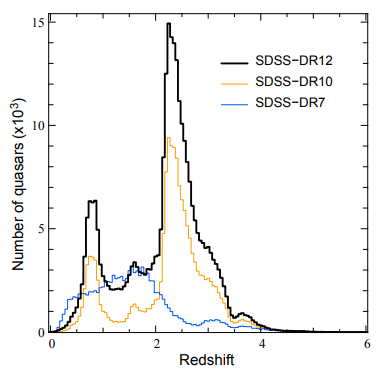
\includegraphics[scale=0.5]{fig/redshift.png}
\caption[Redshift distribution of quasars from the SDSS]{Redshift distribution of the SDSS-DR12 (thick black histogram), SDSS-DR10 (orange histogram) and SDSS-DR7 (blue-histogram) quasars over the redshift range 0-6. The two peaks at $z \sim 0.8$ and $z \sim 1.6$ seen in the SDSS-DR10 and SDSS-DR12 redshift distributions are due to known degeneracies in the SDSS color space \citep{paris2017}.}
\label{fig:qso_z}
\end{figure}


\subsection{Classification and Unification}

Many classes of AGN, names, and terminology appear in literature mainly due to historical observational reasons. To understand the physics and evolution of active galactic nuclei, we usually start with the classification and unification of these objects. 

On the first step, one can differentiate AGNs into radio-loud and radio-quiet sources. To separate radio-loud from radio-quiet AGNs, we can define ``radio-loudness'' parameter, $R$, as fraction between flux density observed at radio 
($S_{\text{radio}}$, at 5 GHz) and at optical wavelength ($S_{\text{optic}}$, at 4400 \AA),
\begin{equation}
R_{ro}  = \frac{S_{\text{radio}}}{S_{\text{optic}}}.
\label{eq:loudness}
\end{equation} 
The dividing line between radio-loud and radio-quiet AGNs is usually set at $R_{ro} = 10$ \citep{kellermann1989}. The next step we can try to distinguish AGN by their emission spectrum/lines, which leads to the so called AGN-\textit{zoo}. Generally, radio-quiet sources can be differentiated into Seyfert galaxies and radio-quiet quasars, while radio-loud sources can be divided into radio-loud quasars, blazars and radio galaxies. 

\begin{figure}[!ht]
\centering
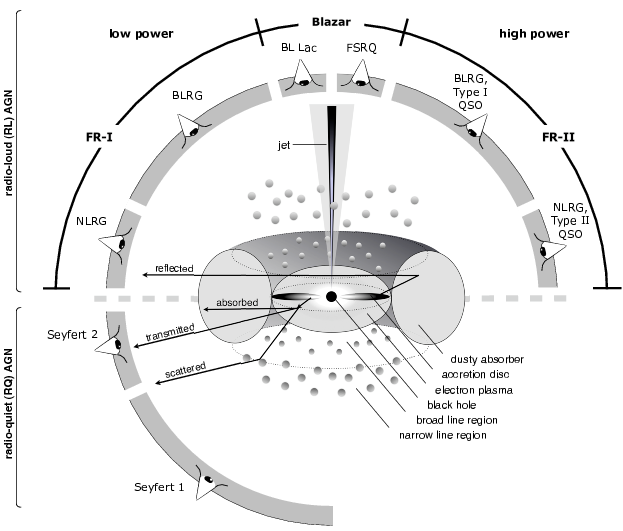
\includegraphics[width=0.85\textwidth]{fig/AGN_unification_Beckmann_Shrader_2012.png}
\caption[Schematic representation of our understanding of the AGN phenomenon in the unified scheme]{Schematic representation of our understanding of the AGN phenomenon in the unified scheme. Graphic by Marie-Luise Menzel, adopted from \cite{beckmann2012}.}
\label{fig:agn_unif1}
\end{figure}

The idea of AGN unification was proposed by \cite{antonucci1993} who suggests that the diversity of AGN can be explained with two parameters: the torus inclination with respect to the line of sight (LOS) and the source luminosity (see \autoref{fig:agn_unif1}). This scheme is perhaps the simplest possible way to characterize the known fact that the nuclear continuum and emission line radiation of AGN can suffer from wavelength-dependent scattering, absorption, and reflection on the way out. This model can account for the different observed properties of emission lines in IR, optical, and UV; the luminosity and variability of the optical-UV continuum; the different amount of obscurity of the central X-ray source. However, it is not as successful in the limits of the very low and very high luminosity, where the presence of such obscurer is questionable \citep{netzer2013}.  

\cite{heckman2014} proposed the next stage of unification model. They classified AGNs into two major groups: radiative-mode AGN and jet-mode AGN. Most of the energy output in radiative-mode AGN is in the form of electromagnetic radiation and is a direct result of matter accretion through a central optically thick accretion disk. On the other hand, jet-mode AGN emit primary energy output in form of bulk kinetic energy transported in two-sided jets. Their typical Eddington ratio is much smaller and jets are most likely powered via radiatively inefficient accretion flows (RIAFs).

In the unified model, radio galaxies and radio-loud quasars both belong to the same parent population \citep{urry1995}. However, there is also an alternative paradigm that recently has been gaining attention in which obscured AGN (e.g. radio galaxies) can evolve into quasar-type AGN as their merger-triggered, dust-obscured AGN become more powerful and clear out the environment \citep[e.g.,][]{hopkins2006}. In this dynamic model, radio galaxies and radio-loud quasars trace different phases in the evolution of powerful AGN and are potentially associated with different environments.

\subsection{Emission Processes}

Radiation sources can be divided into thermal and non-thermal. Thermal emission is produced by a source whose emitting materials are in local thermodynamic equilibrium (LTE). Otherwise, nonthermal emission is produced. Active galaxy or radio galaxy, emit radiation throughout the entire electromagnetic spectrum. The origin of the high-energy emission is still unclear, but in low-energy case or low frequency (e.g., in radio wavelengths), the radiation source (i.e., continuum) is dominated by synchrotron, and dust emission. Only small fraction of energy comes from free-free emission. 

\subsubsection{Synchrotron Emission}

Any accelerated charged particle will emit electromagnetic radiation with power specified by Larmor's formula (nonrelativistic). In astrophysical situations, electromagnetic forces produce the strongest accelerations of charged particles. Acceleration by an electric field accounts for free-free radiation. Acceleration by a magnetic field produces \textit{magnetobremsstrahlung}, the German word for ``magnetic braking radiation''. Electron (and positron if present) is the lightest particle compared to the massive proton/ion. Hence, electrons account for virtually all of the radiation observed.

Consider an electron with energy $E$ that is moving in a uniform magnetic field $B$ of energy density $u_B = B^2/8\pi$. The energy loss rate, $-dE/dt$, which is also the power emitted by the electron, $P$, is given by
\begin{equation}
P = 2 \sigma_T c \gamma^2 \beta^2 u_B \sin^2{\alpha},
\end{equation}
where $\sigma_T$ is the Thomson cross section, $c$ is the speed of light, $\gamma$ is the Lorentz factor, and $\beta = v/c$, where $v$ is the speed of the electron. The angular term $\sin^2{\alpha}$ reflects the direction of motion, where $\alpha$ is the pitch angle between the direction of motion and the magnetic field. Averaging over isotropic pitch angles gives
\begin{equation}
\overline{P} = \frac{4}{3} \sigma_T c \gamma^2 \beta^2 u_B.
\end{equation}

The radiation emitted by a single electron is beamed in the direction of motion. The spectral energy distribution (SED) of this radiation is obtained by considering gyro frequency of the electrons around the field lines ($\omega_B = e B / \gamma m_e c$) and the mean interval between pulses ($2 \pi / \omega_B$). The calculation of pulse width is obtained by considering the relativistic time transformation between the electron frame and the observer frame. This involves and additional factor of $\gamma^2$. Thus the pulse width is proportional to $\gamma^{-3}$ or, expressed in Larmor angular frequency, $\omega_L = e B/ m_e c$, to $\gamma^{-2}$. Fourier transforming these expressions gives the mean emitted spectrum of a single electron, $\overline{P}_{\nu}(\gamma)$, which peaks at a frequency near $\gamma^2 \omega_L$.

Assume now a collection of electrons with an energy distribution ($n(\gamma)d\gamma$) that gives the number of electrons per unit volume with $\gamma$ in the range of $\gamma$ to $\gamma + d\gamma$. The emission coefficient due to electrons can be obtained by summing $\overline{P}_{\nu}(\gamma)$ over all energies
\begin{equation}
j_{\nu} = \frac{1}{4\pi}\int_{1}^{\infty} \overline{P}_{\nu}(\gamma) n(\gamma) d\gamma.
\end{equation}
There is no general analytical solution to this expression since $n(\gamma)$ can take various differents forms. However, there are several cases of interest where $n(\gamma)$ can be represented as a power law in energy $n(\gamma)d\gamma = n_0 \gamma^{-p} d\gamma$. The additional assumption that all the radiation peaks around a characteristic frequency $\gamma^2 \nu_L$, where $\nu_L$ is the Larmor frequency, gives the following solution for $j_\nu$
\begin{equation}
4 \pi j_\nu = \frac{2}{3} \sigma_{T} n_0 u_B \nu_{L}^{-1} \left( \frac{\nu}{\nu_L} \right)^{-\frac{p-1}{2}}
\end{equation}
Consider $p = 2.5$, which is expected in various important cases, for example, particles accelerated by relativistic shocks. This  gives $j_\nu \varpropto \nu^{-0.75}$. To obtain the monochromatic luminosity ($L_\nu$) of an optically thin medium emiting synchotron radiation, we must integrate over the volume of the source,
\begin{equation}
L_\nu = \int_{V} j_\nu dV \varpropto \nu^{-0.75}
\end{equation}
This is similar to the observed continuum slope of many AGNs at radio, optical, UV and X-ray energies (see \autoref{eq:fluxdensity}).

The source of fast electrons can be opaque to its own radiation. This results in a significant modification of the emergent spectrum, especially at low frequencies, where the opacity is the largest. This case is usually called synchrotron self-absorption mechanism and the resulted specific intensity will be proportional to $\nu^{5/2}$, which describes the synchrotron SED at low energies. Concerning this work, using ALMA, this synchrotron radiation can 
be measured in Band 3.

\subsubsection{Dust Emission}

After synchotron, the second most important source of radiation/continuum in low frequencies from an active galaxy is dust emission. All small solid particle in space is called dust grains by astronomers. Interstellar dust was first recognized from their extinction (i.e., scattering and absorption) properties in far-infrared (FIR), optical, and UV wavelengths. Interstellar dust grains are much smaller than common terrestrial dust particles visible to the naked eye, and they are much smaller than the wavelengths $\lambda > 300$ $\mu$m (frequencies $\nu < 1$ THz) accessible to ground-based radio astronomy such as ALMA.

Dust scattering occurs due to oscillating electric field of incident radiation that forces electrons within dust grain to oscillate and, thus, reradiate at the same frequency in all directions.  In the limit $\lambda \gg a$, where $a$ is the size of the grains, these radiators are very inefficient, so their scattering cross section is proportional to $\lambda^{-4}$ (Rayleigh's law). Some of the incident photons are not scattered, but absorbed by the dust grains, which in turn will heat the dust grains. The energy by a single UV photon can significantly raise the temperature of a very small dust grain, so the smallest dust grains are not in thermodynamic equilibrium with the local interstellar radiation field. 

In fact, larger interstellar dust grains have enough heat capacity to come into equilibrium at well-defined temperatures ($20 < T_d({\rm K})<200$), such that the power absorbed is balanced by power reemitted primarily at  FIR wavelengths. At radio wavelengths, the dust absorption contributes much more than dust scattering to the total extinction. One type of galaxy called starburst galaxy, which has very high star formation rate, are very bright in the IR region due to this dust heating process.

%All galaxies are nearly transparent, thus from radio observations, we can see into the dusty starburst galaxies, and the radio luminosity is nearly proportional to the recent rate of star formation, unaffected by dust extinction.

The dusty radio sources do not have Rayleigh-Jeans radio spectra $S_\nu \varpropto \nu^{2}$; they have relatively a spectra rising as $S_\nu \varpropto \nu^{2 + \beta}$ with $1 < \beta < 2$. A striking consequence of such a steeply rising spectrum is that the flux density of a galaxy observed through the atmospheric window (at $\lambda \sim 1$ mm or $\nu \sim 300$, ALMA Band 6 and 7) is nearly independent of its redshift in the range $1 < z < 10$. The strongest submm galaxies tend to be the most luminous, and radio surveys at wavelengths near $\lambda \sim 1$ mm are effective at tracing the rate of star formation over the entire redshift range during which most stars formed \citep[e.g.,][]{blain1993}.

\section{Radio Galaxy}

As previously mentioned, being a member of radio-loud AGN, radio galaxies are types of active galaxy that have enormous radio luminosities \citep[e.g.][]{miley2008, netzer2013, heckman2014}. Because it is luminous, radio-loud active galaxies can be detected at very large distances using the appropriate radio telescopes. Therefore, the distant universe can be probed using these radio-loud active galaxies to provide different information for cosmology. 

The difference between radio galaxy and other member of radio-loud AGN is the resolvable jet structure. The observed structure in radio emission is determined by the interaction between twin jets and the external medium, modified by the effects of relativistic beaming. In optical wavelength they can be divided in two sub-classes: Broad line radio galaxies (BLRG) have emission lines resembling those from Seyfert 1 galaxies, while narrow line radio galaxies (NLRG) have spectra like the Seyfert 2 galaxies. Recently, much work has been done on the effects of these objects on the intergalactic medium, particularly in galaxy groups and clusters. It is important to note that the term radio galaxy in this dissertation will be used not only for the resolvable radio-loud AGN, but for all of them.

\subsection{Morphology}

Unlike quasar, `resolvable radio galaxies' display wide range of radio structures. The most common large scale structures are called lobe, hotspot, jet, and sometime plume (see \autoref{fig:fr}). \textit{Lobes} are roughly ellipsoid structure, usually double and fairly symmetrical on either side of nucleus. In rather low luminosity case, it is often called \textit{plumes}. Some radio galaxies show one or two narrow features known as \textit{jets}, directly coming from nucleus and going to the lobes. It is believed that lobes or plumes are powered or supplied by high-energetic particles and magnetic fields from active nucleus through this jets \citep[see, e.g., ][]{scheuer1974, blandford1974}.

\begin{figure}[!ht]
\centering
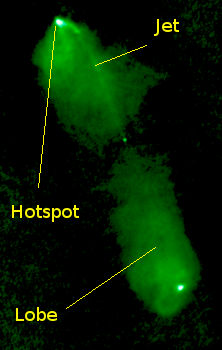
\includegraphics[width=0.49\textwidth]{fig/Radio_galaxy_3C98.png}
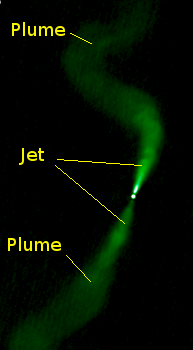
\includegraphics[width=0.425\textwidth]{fig/Radio_galaxy_3C31.png}
\caption[Example of radio image for the FR I and FR II radio galaxy]{(Left) Radio image of FR II radio galaxy, 3C98. (Right) Radio image of FR I radio galaxy, 3C31. Labelled in the image are structures usually found in radio galaxy: lobes, jets, hotspot, and plumes.}
\label{fig:fr}
\end{figure}

\cite{fanaroff1974} divided radio galaxies into two clasess based on their morphology, i.e., FR I and FR II. While FR I are radio galaxies that have brighter spot located at the center of active nuclei and gradually decrease, FR II are radio galaxies that have brighter spots located at the far edge of the jet/lobes. Furthermore, \cite{fanaroff1974} found that FR II are more luminous than FR I. In some cases, we cannot classify the class of radio galaxy, either as FR I or FR II. On the other hand, there is a hybrid case in which FR I is seen on one lobe and FR II on the other lobe. With more detailed radio observations, the morphology reflects the mechanism of energy transport in the radio source. Consequently, the environment of radio galaxies plays important roles.

It also has been argued that FR II radio galaxies, are triggered by molecular gas fed towards the center \citep{buttiglione2010}, while the FR I type are triggered through a ``dry'' accretion (Bondi accretion) in the Broad Line Region (BLR, see \citep{fromerth2001}). A key aspect is the ability to feed the accretion disk around the central Supermassive Black Hole (SMBH, see \cite{merloni2008}). It has been suggested that ``wet'' minor mergers would be a mechanism to bring molecular gas and dust towards the center of the radio galaxies and trigger the radio activity \citep[e.g.,][]{lim2000, israel1998}.

\subsection{Host Galaxies and Environments}

Observations have shown that radio-loud AGN usually reside in overdense environments \citep[see, e.g.,][]{stevens2003, venemans2007, falder2010, galametz2010b, galametz2012, mayo2012}. The host galaxies are almost exclusively large and massive elliptical galaxies. If the radio jets are not in the LOS, the central black hole in radio galaxies is usually obscured by a thick dust torus and does not outshine the host galaxy. Therefore, investigating the SED of radio galaxies enables one to study their host galaxy's stellar, dust and AGN components. Nevertheless, for a distant-unresolvable radio galaxy, it will be difficult to disentangle these components, because we don't have any information about the orientation of the radio jet.

Radio galaxies are very luminous in FIR regime indicating very high star-formation rates. Observations show that star-formation rates in radio galaxies can reach several thousands $M_{\odot}$/yr \cite[e.g.,][]{archibald2001, drouart2014}. Moreover, \cite{miley2008} found that their sub-millimeter luminosity increases with redshift, implying that star-formation rates were higher at early times. Nevertheless, it is also difficult to disentangle the source of dust heating process: by AGN or stars. It requires detailed modelling and SED fitting of each component. Observation on Rayleigh-Jeans tail of the sub-millimeter region is crucial as it may constrain the slope of the dust emission heated by stars \citep{drouart2014}. This tail is also important for deriving far-infrared photometric redshifts \citep{wylezalek2013b}.  ALMA frequency is important because it is located in this region. Catalogue of SED produced in this work will be useful to disentangle the source of dust heating process in radio galaxies, which will then be useful to correctly measure the star formation rates.


% Equally interesting is their likely effect on structure formation over cosmological time: it is thought that they may provide a feedback mechanism to slow the formation of the most massive objects.

\cleardoublepage

\chapter{Radio Interferometry}

Since this work analyzes mostly data from radio observations, in particular using interferometer array, in this chapter we briefly review some basic concepts of radio interferometric observations. We also describe some basic properties of the ALMA radio telescope.  

The angular resolution ($\theta_{\text{res}}$) of single dish radio telescope is given by 
\begin{equation}
\theta_{\text{res}} = 1.22\ \frac{\lambda}{D},
\label{eq:thetares}
\end{equation}
where $\lambda$ is the wavelength and $D$ is the diameter of the telescope. The intensity distribution of an incoming signal can be calculated by using a Bessel's function, so that the approximation of the first Bessel's function becoming zero leads to the numerical factor of 1.22. 

For the same diameter size, observations in longer wavelength (radio) result in a smaller angular resolution. To improve the angular resolution for an observation at a given wavelength, the diameter of the telescope has to be increased. Fortunately, in radio wavelenths, this can be done by synchronization of multiple radio telescopes called radio interferometry techniques. The resolution of the system is comparable to the distance of the longest baseline, i.e., the farthest distance between two telescopes.

\section{Aperture Synthesis}

The simplest array of telescopes consists of two identical antennas, hence the concept of radio interferometry can be explained with much simplification by the so called two-element interferometer (\autoref{fig:twoline}). The following explanations and descriptions are adapted from \cite{burke2014} and ALMA Technical Handbook \citep{almatech2016}.

\begin{figure}[!ht]
\centering
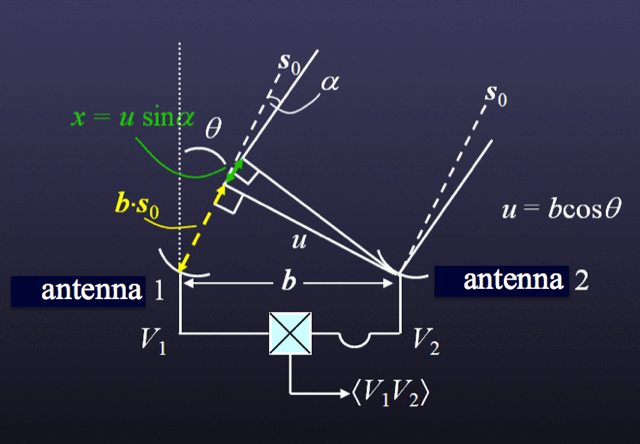
\includegraphics[width=0.7\textwidth]{fig/baseline.png}
\caption{Two-element interferometer, consists of two antennas. Ilustration from ALMA Technical Handbook (\citeyear{almatech2016}).}
\label{fig:twoline}
\end{figure}

The power received by one single telescope/element is given by
\begin{equation}
P = \int_{0}^{\infty} A_{\text{eff}}(\nu) S(\nu) d \nu,
\end{equation}
where $S(\nu)$ is the flux density of the source, given by its brightness distribution integrated over the solid angle, and $A_{\text{eff}}(\nu)$ is the effective area of the dish. In the radio interferometry, this power is converted into voltage. Since the power is proportional to the square of voltage, to recover the flux receive from the source, we need to multiply the voltage response from each antenna (that is, auto-correlation and cross correlation).

\autoref{fig:twoline} shows a schematic diagram of a two-element interferometer separated by a distance $L$. We can measure this distance in units of the observing wavelength ($\lambda$), $b = L/\lambda$, usually called baseline. Both antennas observe a common position $s_0$ located at an angle $\theta$ from the meridian. The projected separation of the two antennas towards $s_0$ from the perspective of the source is $u = b \cos \theta$. The signal arrives at the first antenna delayed by the geometrical delay $\tau_g = \frac{b \cdot s_0}{c}$. To compensate for the geometrical delay, an artificial delay can be inserted into the signal path of antenna 2 (e.g., electronically) so that the signals from both antennas arrive at the correlator with the same phase.

Moving slightly off-axis, we can describe a small angle from the axis as $\alpha$, and its 1-D sky position as $l = \sin \alpha$. At angle $\alpha$, an off-axis signal reaching antenna 1 will have to travel a slightly longer path than an off-axis signal reaching antenna 2, even with the geometrical delay introduced to compensate for an on-axis signal. This extra path length is $x = u \sin \alpha = ul$. It turs out that the extra path lengths result in phase differences with $\alpha$ that can be characterized where the voltage response of antenna 2, $V_2$, can be written in terms of the product of the voltage response of antenna 1, $V_1$, and a phase delay factor sinusoidally varying as a function of angle, that is,
\begin{equation}
V_2 = V_1 e^{2 \pi i u l}
\end{equation}

In 2-D case, we can define similar angle in orthogonal direction, and the equation becomes
\begin{equation}
V_2 = V_1 e^{2\pi i (ul + vm)},
\end{equation}
where $u$ and $v$ is called specific spatial frequency components of the sinusoid in the East-West and North-South directions, respectively, and these are the projected lengths of the antenna separations measured in units of the wavelength at the time of observation. In addition, we identify $l$ and $m$ as direction cosines relative to a reference position in the E-W and N-S directions, respectively. The on-axis position $s_0$ has $l = 0$ and $m = 0$ and is called the phase center.

The correlator acts as a multiplying and time-averaging device for the incoming signals from antennas 1 and 2,
$$\left\langle V_1 V_2 \right\rangle = \left\langle \int\int V_1 (l,m) dl dm  \int\int V_2 (l,m) dl dm \right\rangle$$
Under the assumption that signals emanating from different parts of the sky are incoherent, the time averages of the correlation of those signals will be zero. Thus, the product of the integrals can be simplified into the form 
\begin{eqnarray}
\left\langle V_1 V_2 \right\rangle &=& \left\langle \int\int V_1 (l,m) V_2 (l,m) dl dm \right\rangle \\
&=& \int\int \left\langle V_1 (l,m)^2 \right\rangle e^{2 \pi i (ul + vm)} dl dm \\
&=& \int\int I(l, m) e^{2 \pi i (ul + vm)} dl dm 
\end{eqnarray}
where $I(l, m)$ is the intensity distribution on the sky. The correlator therefore measures a quantity known as the ``complex visibility'', $\mathcal{V}$, which is formally the Fourier transform of the intensity distribution on the sky:
\begin{equation}
\mathcal{V}(u,v) = \int \int I(l, m) e^{2 \pi i (ul + vm)} dl dm = A e^{i\phi}
\end{equation}
$\mathcal{V}$ is a complex number, and can be described by an amplitude $A$ and a phase $\phi$. The amplitude and phase contain information about the source brightness and its location relative to the phase center, respectively, at spatial frequencies $u$ and $v$.

The relationship between the sky brightness distribution and the complex visibility distribution is governed by the \textit{van Cittert-Zernike theorem} which says that ``Complex visibility is the Fourier transform of the sky brightness distribution in the image plane''. It is the basis of the aperture synthesis.

It follows that ``the sky brightness distribution is in turn the inverse Fourier transform of the complex visibility distribution in the visibility plane'' or $uv$-\textit{plane}.
\begin{equation*}
I(l, m) = \int \int \mathcal{V}(u, v) e^{-2 \pi i (ul + vm)} du dv 
\end{equation*}

Theoretically, by measuring all of the \textit{complex visibilities}, we can reconstruct the true sky brightness. However, in reality not all of $uv$-plane can be sampled because of the limit on the number of the antenna or baseline combination. 

To reconstruct the true sky brightness we need to use \textit{deconvolution} technique, usually called  `CLEAN'ing procedure. Moreover, due to incompleteness of spatial frequency sampled from observation, we need to choose the configuration of the antenna array that can recover at maximum the features or details seen on the target object. To recover small features, we need more sparse array configuration. On the other hand, we need more compact configuration to recover large features of the target. 


\section{Atacama Large Millimeter/submillimeter Array (ALMA)}

The Atacama Large Millimeter/submillimeter Array (ALMA) is a new facility of radio interferometer array consisting of 66 
antennas (that is, 54 antennas of the 12-m diameter and 12 antennas of the 7-m diameter) that can be arranged in a series of 
different configurations, covering a baseline of a few meters up to 18 km. The ALMA 
antennas are located on the Chajnantor Plateau, Chile (lat. = -23.02917$^{\circ}$, long. = -67.754649$^{\circ}$)
at the altitude of 5000 m. Therefore, this site represents one of the driest place in the world (see \autoref{fig:ALMAtransmission}) 
and is very suitable to host radio telescopes that can
operate over a broad range of observing frequencies in the millimeter and submillimeter range. ALMA Early Science 
Operations started with Cycle 0 in September 2011 (with less than 20 antennas) and the official inauguration took place in March 2013. 
Long baseline campaigns have been started in Cycle 3 and succesfully yielded many remarkable results. After subsequent
development, ALMA presently works in Cycle 4 with more advanced capability. 

\begin{figure}[!ht]
\centering
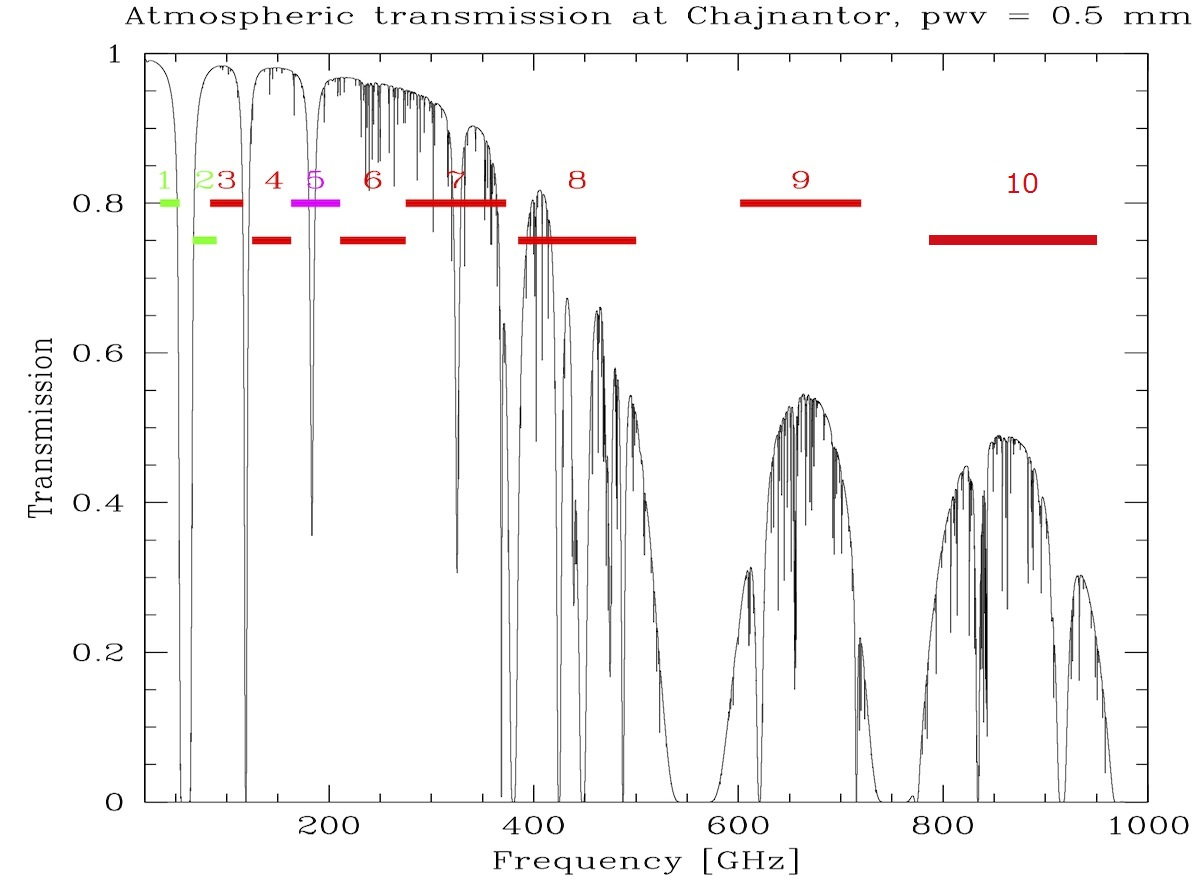
\includegraphics[width=0.99\textwidth]{fig/transmission.png}
\caption[ALMA receiver bands for Cycle 4 (2017)]{The ten ALMA receiver bands. Receiver bands for Cycle 4 (2017) are shown in red superimposed on a zenith atmospheric transparency plot for 0.5 mm of PWV.}
\label{fig:ALMAtransmission}
\end{figure}

\begin{table}[!ht]
\centering
\caption[ALMA receivers characteristics.]{ALMA receivers characteristics. Band 1 and 2 are still in the development process, Band 4, 9, 10 are only operated recently, Band 5 not used for science. Configuration, SSB: single sideband; 2SB: both sidebands detected separately; DSB: double sideband.}
\label{tab:ALMAreceiver}
\begin{tabular}{ccccc}
\hline
Band   & Frequency Range & Wavelength & Instantaneous   & Config \\
Number & (GHz)           & (mm)       & Bandwidth (GHz) &               \\
\hline
1      & 31.3 -- 45.0     & 6.7 -- 9.6  & 1 $\times$ 8           & SSB           \\
2      & 67 -- 90         & 3.3 -- 4.5  & 1 $\times$ 8           & SSB           \\
3      & 84 -- 116        & 2.6 -- 3.6  & 2 $\times$ 4           & 2SB           \\
4      & 125 -- 163       & 1.8 -- 2.4  & 2 $\times$ 4           & 2SB           \\
5      & 163 -- 211       & 1.4 -- 1.8  & 2 $\times$ 4           & 2SB           \\
6      & 211 -- 275       & 1.1 -- 1.4  & 2 $\times$ 5.5         & 2SB           \\
7      & 275 -- 373       & 0.8 -- 1.1  & 2 $\times$ 4           & 2SB           \\
8      & 385 -- 500       & 0.6 -- 0.8  & 2 $\times$ 4           & 2SB           \\
9      & 602 -- 720       & 0.4 -- 0.5  & 2 $\times$ 8           & DSB           \\
10     & 787 -- 950       & 0.3 -- 0.4  & 2 $\times$ 8           & DSB   \\
\hline
\end{tabular}
\end{table}

The ALMA front end can accommodate up to 10 receiver bands (\autoref{tab:ALMAreceiver}) covering most of the 
wavelength range from 10 to 0.3 mm (30 \--- 950 GHz). Each receiver band is designed to cover atmospheric transmission 
windows in this range of frequency (\autoref{tab:ALMAreceiver}). The angular resolution can reach up to $0.02''$ 
(for example, at $\lambda = 1$  mm and 10 km baseline), with the baseline range from 15 m to 18 km. \autoref{fig:ALMAtransmission} shows 
the atmospheric transmission in ALMA site with a typical precipitable water vapour (PWV) of 0.5 mm 
together with the coverage of ALMA observing bands. As previously mentioned, 
the receiver bands that have strong interest in this work are Bands 3, 6, 7, and 9. We can `see' the synchrotron radiation in Band 3, on the other hand Band 6, 7, and 9 usually used to `see' the dust emission from the galaxy. 


%\subsubsection*{ALMA Cycle and Data}
%\begin{itemize}
%\item Cycle 0
%\item Cycle 1
%\item Cycle 2
%\item Cycle 3
%\end{itemize}

\cleardoublepage

\chapter{Data Selection and Analysis}

Every ALMA science project incorporates calibration observations of radio sources, which are mostly radio galaxies, to set various observational parameters of the science targets. These calibrations comprise the determination of bandpass, flux, and phase calibrations that lead to correct estimation of visibilities of the science targets. Therefore, multiple observations of ALMA calibrators must be made for each project.  

In this work, we will exploit the large amount of calibrators data acquired by ALMA, during its operation. By combining accumulated compatible data, we should be able to reach a sufficiently low noise level to obtain deep image to detect the environment of radio galaxies. Our target is to gather the maximum number of calibrators ($>20$) and make the deepest image so far in continuum for the ALMA bands available during the undertaking of this work. Some previous results have been demostrated in \cite{leon2016}.

The data are most likely acquired from Bands 3, 4, 6, 7, 8, and 9, accumulated from Cycle 1 to present. The data from Cycle 0 were not considered due to the use of smaller number of antennas during observations, leading to lower dynamic ranges. By automatizing at maximum the data reduction: downloading, self-calibration, concatenation, image ``cleaning'', and filtering, we should be able to study several radio galaxies in the range of redshift ($z$) from 0 to 2 with a very deep sensitivity of the order of a few tens of $\mu$Jy.


\section{Data Selection}
%\subsubsection{Selection Criteria}
To search for the calibrators utilized by ALMA to conduct their science programs, 
the ALMA Source Calibrator Catalogue (\url{https://almascience.eso.org/sc/}) is avalable and can be checked regularly. 
Subsequently, to obtain the corresponding data, one can access the ALMA Science Archive Query (\url{almascience.nrao.edu/aq}) 
to browse all the observations or projects 
that utilize the corresponding objects as calibrators. We have been using \textsf{astroquery.alma} to access and compile 
information from the ALMA Archive Database. 
For the first selection, we introduce specific criteria based only on the data availability, i.e., 
\begin{itemize}
\item Ignoring data from Cycle 0 due to the small number of antennas and the unfixed data structure
\item Neglecting polarization product and frequency resolution
\item Considering only observations using the 12m array 
\item Total integration time is sufficiently long, particularly in Bands 3, 6, and 7 
\item Publicly available data only 
\end{itemize}

\begin{table}
\caption{Selected ALMA calibrator based on data availability (query as of 10 April 2017).}
\begin{tabular}{lccccccccc}
\hline
Calibrator & $z$ & Flux (Jy) & \# projects & B3 & B4 & B6 & B7 & B8 & B9 \\
\hline
J0241-0815	&	0.005			&	1.003	&	22	&	1.1	&		&	1.8	&	3.5	&	0.5	&		\\
J0348-2749	&	0.991			&	0.73	&	23	&	1.1	&	0.3	&	1.8	&	2.8	&	0.1	&	0.1	\\
J0635-7516	&	0.653			&	1.41	&	25	&	1.3	&		&	3.1	&	1.1	&		&		\\
J0854+2006	&	0.3056			&	7.27	&	28	&	1.5	&	0.1	&	1.5	&	2.5	&		&	0.4	\\
J2253+1608	&	0.859			&	9.17	&	30	&	1.9	&	0.2	&	1.4	&	1	&	0.5	&	1.1	\\
J0006-0623	&	0.3467			&	4.163	&	32	&	1.4	&	0.2	&	1.1	&	2.9	&	0.4	&		\\
J1550+0527	&	1.422			&	0.97	&	34	&	2.8	&	0.3	&	2.1	&	2.6	&		&	0.8	\\
J1617-5848	&	1.422			&	1.11	&	35	&	4.6	&	0.2	&	1.9	&	1.9	&	0.1	&	0.1	\\
J2148+0657	&	0.99			&	1.6	&	41	&	1.2	&		&	3.5	&	3.6	&	1.1	&	0.5	\\
J2232+1143	&	1.037			&	6.29	&	43	&	1.9	&	0.2	&	1.1	&	3.5	&	1.8	&	0.4	\\
J0538-4405	&	0.894			&	1.98	&	46	&	2.2	&		&	3.8	&	2.9	&		&		\\
J0519-4546	&	0.035			&	1.27	&	47	&	3.9	&	0.7	&	4	&	1.6	&		&	0.1	\\
J0522-3627	&	0.0565			&	7.13	&	51	&	1.4	&		&	1.7	&	11.3	&	1	&	1.7	\\
J1337-1257	&	0.539			&	3.25	&	51	&	2.6	&	0.2	&	1.9	&	4.2	&		&	0.8	\\
J1229+0203	&	0.1583			&	10.05	&	57	&	3.3	&	0.5	&	4.5	&	3.7	&	0.5	&	0.8	\\
J1107-4449	&	1.598			&	1.06	&	58	&	3.4	&		&	4.1	&	1.3	&		&		\\
J1037-2934	&	0.312			&	2.28	&	59	&	1.6	&	0.6	&	3.6	&	3.3	&	0.1	&	0.5	\\
J1256-0547	&	0.5362			&	10.91	&	60	&	1.9	&	0.3	&	3.6	&	4.6	&	2.7	&	5.2	\\
J0238+1636	&	0.94			&	2.19	&	67	&	1.7	&	0.3	&	3.4	&	1.9	&	0.4	&		\\
J1517-2422	&	0.049			&	2.1	&	71	&	1.8	&	0.2	&	4.5	&	13.7	&	0.3	&	0.1	\\
J2258-2758	&	0.926			&	2.21	&	73	&	4.3	&	0.4	&	8	&	2.2	&	0.3	&	0.2	\\
J1427-4206	&	1.522			&	3.21	&	74	&	4.7	&		&	3.3	&	8.1	&	0.8	&	1.5	\\
J1058+0133	&	0.89			&	5.39	&	86	&	5	&	0.3	&	5.9	&	12.1	&	0.3	&	0.4	\\
J1924-2914	&	0.3526			&	5.6	&	87	&	2.7	&	0.4	&	5.5	&	11.9	&	2.1	&	2.3	\\
J1733-1304	&	0.902			&	2.91	&	87	&	4.6	&	0.7	&	12.4	&	6.2	&	0.1	&	0.3	\\
J0334-4008	&	1.445			&	0.9	&	103	&	8.2	&	2.9	&	10.2	&	4.9	&	0.4	&	1.6	\\
J0423-0120	&	0.9161			&	0.93	&	104	&	4.5	&	0.4	&	8.8	&	8.5	&	0.1	&	0.2	\\
\ldots	&	\ldots			&	\ldots	&	\ldots	&	\ldots	&	\ldots	&	\ldots	&	\ldots	&	\ldots	&	\ldots	\\
\hline
\end{tabular}
\label{tab:selectedcalibrator}
\noindent Notes: Columns B3 --- B9 are the total integration time (in hours) in the corresponding Bands 3 to 9, 
if we combine all the data from all the available projects. 
\end{table}

Based on these criteria, for example, if we require the total integration time longer than one hour for each Band 3, 6, 
and 7, then we can obtain 27 objects satisfying our requirement. Combining all of them, Table \ref{tab:selectedcalibrator}
presents the list of these 27 calibrators acquired from all the projects with the corresponding total integration time
(query as of 10 April 2017).
Redshifts ($z$) shown in Table \ref{tab:selectedcalibrator} are incorporated from  the NED website (NASA/IPAC {\it Extragalactic Database}, 
\url{http://ned.ipac.caltech.edu/forms/denv.html}). Flux in this table is taken from Band 3 and it may fluctuate significantly 
from days to weeks. \autoref{flowchart:dataselection} shows the detailed data selection process using a flowchart.

\begin{figure}[ht]
\centering
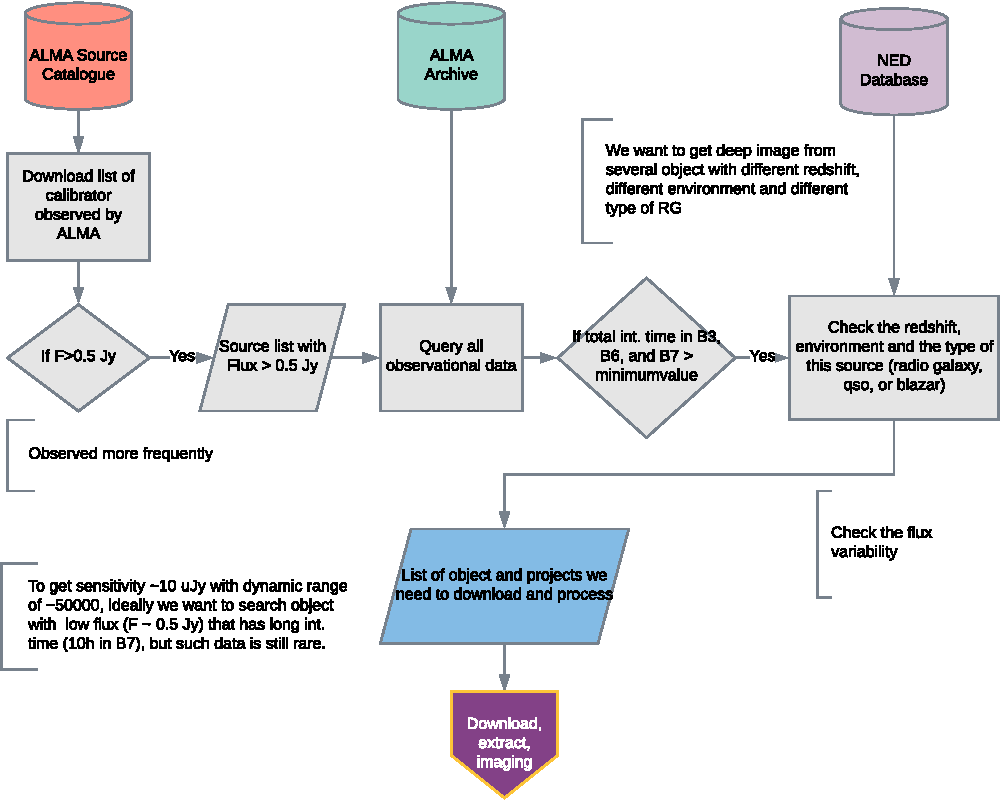
\includegraphics[width=\textwidth]{fig/selection-crop.pdf}
\caption{Flowchart of the data selection process.}
\label{flowchart:dataselection}
\end{figure}

For the second selection, concerning to study the environments of radio galaxies, we introduce further criteria 
for the objects based on their physical properties, i.e., (1) 
there are sources which are relatively isolated and other sources that are located in a group or clusters (in environment
of galaxies); and also (2) the selected samples should have different redshifts. However, such selection criteria are currently not 
applicable yet because of the still limited data available in public domain. 
Since the first goal of this research is to build a catalagoue or database of the point 
sources around the calibrators (radio galaxies), we apply the first selection criteria to retrieve the maximum number of
objects matching our criteria.  
Furthermore, considering our first results, we will conceive in-depth study from samples of radio galaxies based on 
the environment condition. We also envisage to write proposals of follow up observations following the results obtained.

%\subsubsection{Data Format and Limitation}

\section{Method}

Once the data are in public domain,  we can use these data from the ALMA archive through a selection process according to our defined science goals or constraints described above. However, care must be taken since every ALMA science project contains very big data. Typical data sizes from Cycle 1 and later are 25 -- 200 Gb for each science project before further processing (in tarred and zipped files). Sometimes, they are even bigger depending on the types of  the project, number of antenna, and time of integration. Data processing and further analyses will typically need more than 1 Tb disk size for one ALMA science project. Hence, one aspect of this work concerns about big data handling. We note that hundreds of ALMA science project will be selected during this work.

The {\it Common Astronomy Software Applications} package \citep[CASA, ][]{casa} is entirely used in this work to process the ALMA data. After downloading the raw data, we should perform the calibration from the ASDM file (ALMA Science Data Model) yielding
measurement set (MS) that is ready to process further. Generally, the final product is image as well as spectrum of the object. 

The data can be analyzed or processed individually and, subsequently, may be concatenated from several observations or bands. 
Note that one of the technical 
aspects in this work is to improve the dynamic range of the resulted image using wavelet filtering and detection of the 
point sources and absorption lines (different kernels) as well as to automatize the self-calibration. A first testbed was 
successfully applied to the calibrator PKS 0521-365, described in \cite{leon2016}.

\subsection{Splitting and Self-Calibration}

In details, we repeate the procedure here.
After selecting a calibrator, we can start by downloading the related project. Then, we split the data after converting it 
from ASDM to MS. For each project, usually there are three to four different objects observed as calibrators. Next, we collect 
all the calibrator data. Some of them 
may be used later since they were also selected in our source/calibrator list. Then the remaining data can be deleted to save the 
space disk. We remind that we deal with huge data.  

The splitted calibrator MS need to be self-calibrated. Self-calibration procedure is performed to increase the effective sensitivity 
of the image. This can be done by introducing a model of our source. We solve for the calibrations that best match 
our data to our model. We can get a model of our source through an initial image of our source. Self-calibration is 
recommended if the source have high enough signal-to-noise ratio (SNR), e.g., $> 20$ in our initial image. There are 
two types of self-calibration: phase (p) and amplitude-phase (ap). We already did some tests using our data and agreed 
to do three step of self-calibration, i.e. phase, phase, and then amplitude-phase calibration, to maximize the 
sensitivity or minimize the root-mean-square (rms) noise of the image ($\sigma$).

After self-calibration, we substract the image with a point source model in the location of calibrator. Substraction 
is done in the $uv$-plane, not in image plane. Substraction must be done to reduce the effect from the variability of 
the calibrator or central source to the (e.g. flux) environmental source that we want to extract and analyze. The whole procedure
is briefly shown in \autoref{fig:selfcal} using a flowchart. 

\begin{figure}[ht]
\centering
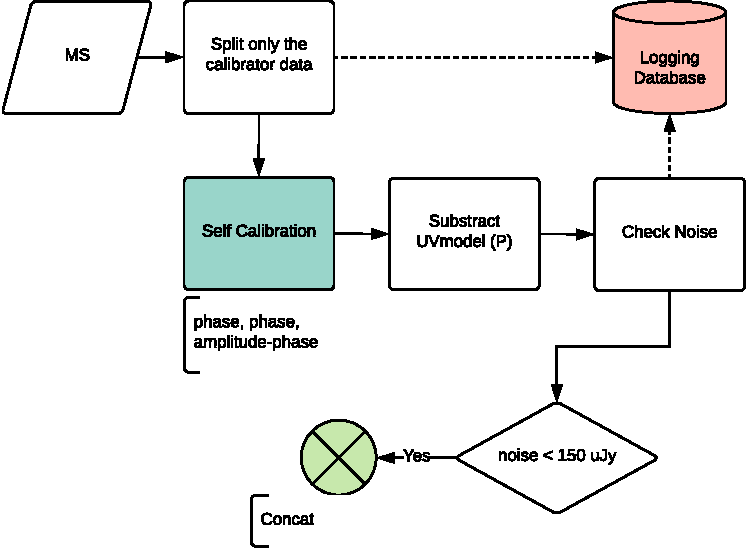
\includegraphics[width=0.8\textwidth]{fig/selfcal-crop.pdf}
\caption{Flowchart of collecting the calibrator data and self-calibration.}
\label{fig:selfcal}
\end{figure}

\subsection{Concatenating}

After collecting all the self-calibrated-substracted-MS of the calibrator, we can start to concatenate the data. 
Concatenating will increase the sensitivity of the final image. Each observation of a calibrator may only takes $3-6$ 
minutes, but if we can concatenate all the data from ALMA Archive, we can get a data with the total integration 
time up to several hours, without conducting a dedicated observation. It is worth noting that to concatenate image data, 
(1) we should not include bad data (after inspection, since they will not help to increase the SNR), 
(2) we can use a weighting based on the rms-noise of each initial images.

The pipeline to do the above processes have been developed, but some work has yet to be done to improve it. 
The example of point source that we 
successfully performed to extract the appropriate data using our pipeline is 
shown in \autoref{fig:test_J0241-0815_B7}. We notice that the detection of a very bright point 
source, at more than 10$\sigma$ level, can be identified at RA: $02^{h}41^{m}04.82^{s}$ and DEC: $-08^{\circ}15'15.0''$ (J2000) 
in northern part of the 
calibrator J0241-0815. This result is consistent with the similar work from ALMACAL team \citep{almacal1_2016}. 
We also detect a dim counterpart of that source in Band 3 and 6.

\begin{figure}[ht]
\centering
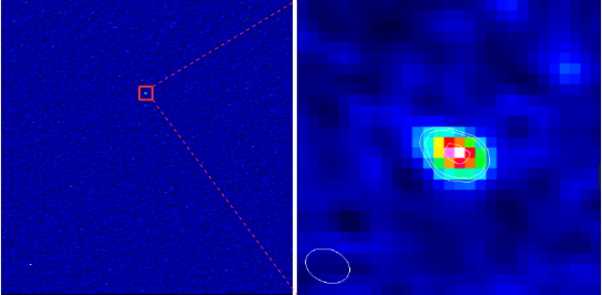
\includegraphics[width=\textwidth]{fig/J0241-0815_test.png}
\caption[First result of the workflow for the calibrator J0241-0815 in ALMA Band 7.]{Calibrator J0241-0815 in Band 7 (located at the center of left panel). We split this calibrator from the project, do self-calibration, subtract with a point source model, and then concat the resulted MSs. This image results from the combined data of 5 MSs, reducing the RMS noise level from $\sim$90 $\mu$Jy to 53 $\mu$Jy. We detect a point source in the the environment of this calibrator (see a zoom in feature in right panel). White contours represents $5\sigma$, $6\sigma$, and $10\sigma$ noise level, respectively.}
\label{fig:test_J0241-0815_B7}
\end{figure}

\section{Analysis}

To produce the catalogue of the point source emission in and around these radio galaxies from the final data/image, we will use a well-controlled image analysis software, e.g., SExtractor (\url{http://www.astromatic.net/software/sextractor}). The real point source may be identified in different frequencies/bands. This also can be used to produce the Spectral Energy Distribution (SED) of the source. If the source is not detected in all the bands, we need to be careful, since it might be either a real source or spurious data. Further analysis can be done by comparing the image with the observation from other range of electromagnetic observations, especially from other radio survey, optical, infrared, and X-ray. These additional data can be an image or a catalogue in the calibrator sky-region. Some related survey/archive that can be used such as SDSS, Hyper Suprime-Cam Subaru, MAST ( Multimission Archive at STScI), NED, Galex, Spitzer, WISE, and FIRST (Faint Images of the Radio Sky at Twenty-cm) survey. The corresponding information can be used to verify the point source detection and also to determine the SED of the object. It is important to check the quality of the final data/image by performing statistical tests, such as completeness test. We can also improve the dynamic range of the image using wavelet filtering.

The final output of the Ph.D thesis will be a very deep catalogue of the dust emission in and around radio galaxies to analyze the environment effects on the ISM content in these objects. This catalogue may include several parameters such as SED, spectral index, dust mass, and dust temperature. If the sample of calibrator/radio galaxy is large enough, we can see the effect of the galaxy evolution through the cosmic time (redshift) i.e. interplay between the activity of the central engine of radio galaxy (SMBH), star formation rates in the host galaxy, and the environment of the radio galaxy galaxy. The synchrotron emission (radio jets) with the high angular resolution will be analyzed, in particular its interaction with the dust in the host elliptical galaxies. We can measure the synchrotron emission using ALMA band 3, because the peak of this emission is in lower frequency (below 20 GHz), while the dust can be measure using ALMA band 6 and 7. 

The analysis of these data will be completed by the study of absorption lines towards the strong continuum of the radio galaxies to study the molecular gas content. These absorption lines in majority are expected from our own Galaxy, therefore this data will be important for mapping the molecular gas in our Galaxy.


\cleardoublepage

\chapter{Work Plan}

To accomplish the objective of this doctoral research, we compose the work plan for our time line that generally consists of:

\begin{enumerate}

\item Data acquisition and data processing of several radio galaxies from ALMA calibrator public data

\item Developing the automation script to analyze new incoming ALMA's calibrator data 

\item Analyzing the data to derive some basic parameters of radio galaxy in (sub)mm region and improving the dynamic range of 
the corresponding image

\item Analyzing the data and the environment of radio galaxies incorporating the observational data from other wavelenghts

\end{enumerate} 

We note that some works in developing the automation scripts have been completed and they were used to process about 10 sources. More sources are certainly in progress. Since this work is in a cooperation framework with the JAO, some parts of the jobs is previewed to be conducted in ALMA Santiago Center Office (SCO), Chile. A short visit in 2017 (4 months), from April to July, has allowed to complete the basic tools necessary for the job. Next visit in the scheme of ESO Studentship is planned from April 2018 to April 2019. 

In dealing with huge data such as ALMA science projects, we certainly needs good infrastructures, namely a reliable internet connection, computer clusters, sufficient disk space, and reliable laptops. Fortunately, this facility can be provided more or less adequately. When we stay in Santiago, we use the ALMA Cluster (almascoop) which is avalable almost permanently. In ITB, we use Perseus Cluster (running with 16 processor) and another Workstation (running with 8 processors). An ordinary Linux desktop (with i3 processor) is also avalable to share the job. In total, we have approximately 15 Tb of space disk available to conduct this work, albeit some space must be shared with others. We are also granted from the ITB Network Administration an unlimited quota of internet connection to conduct this work.  

It remains to find an effective and efficient way to manage the transfer of these huge data between different machines in order to allow saving time. The timeline describing those steps are shown in \autoref{fig:workplan}.


\begin{landscape}
\begin{figure}[!ht]
\centering
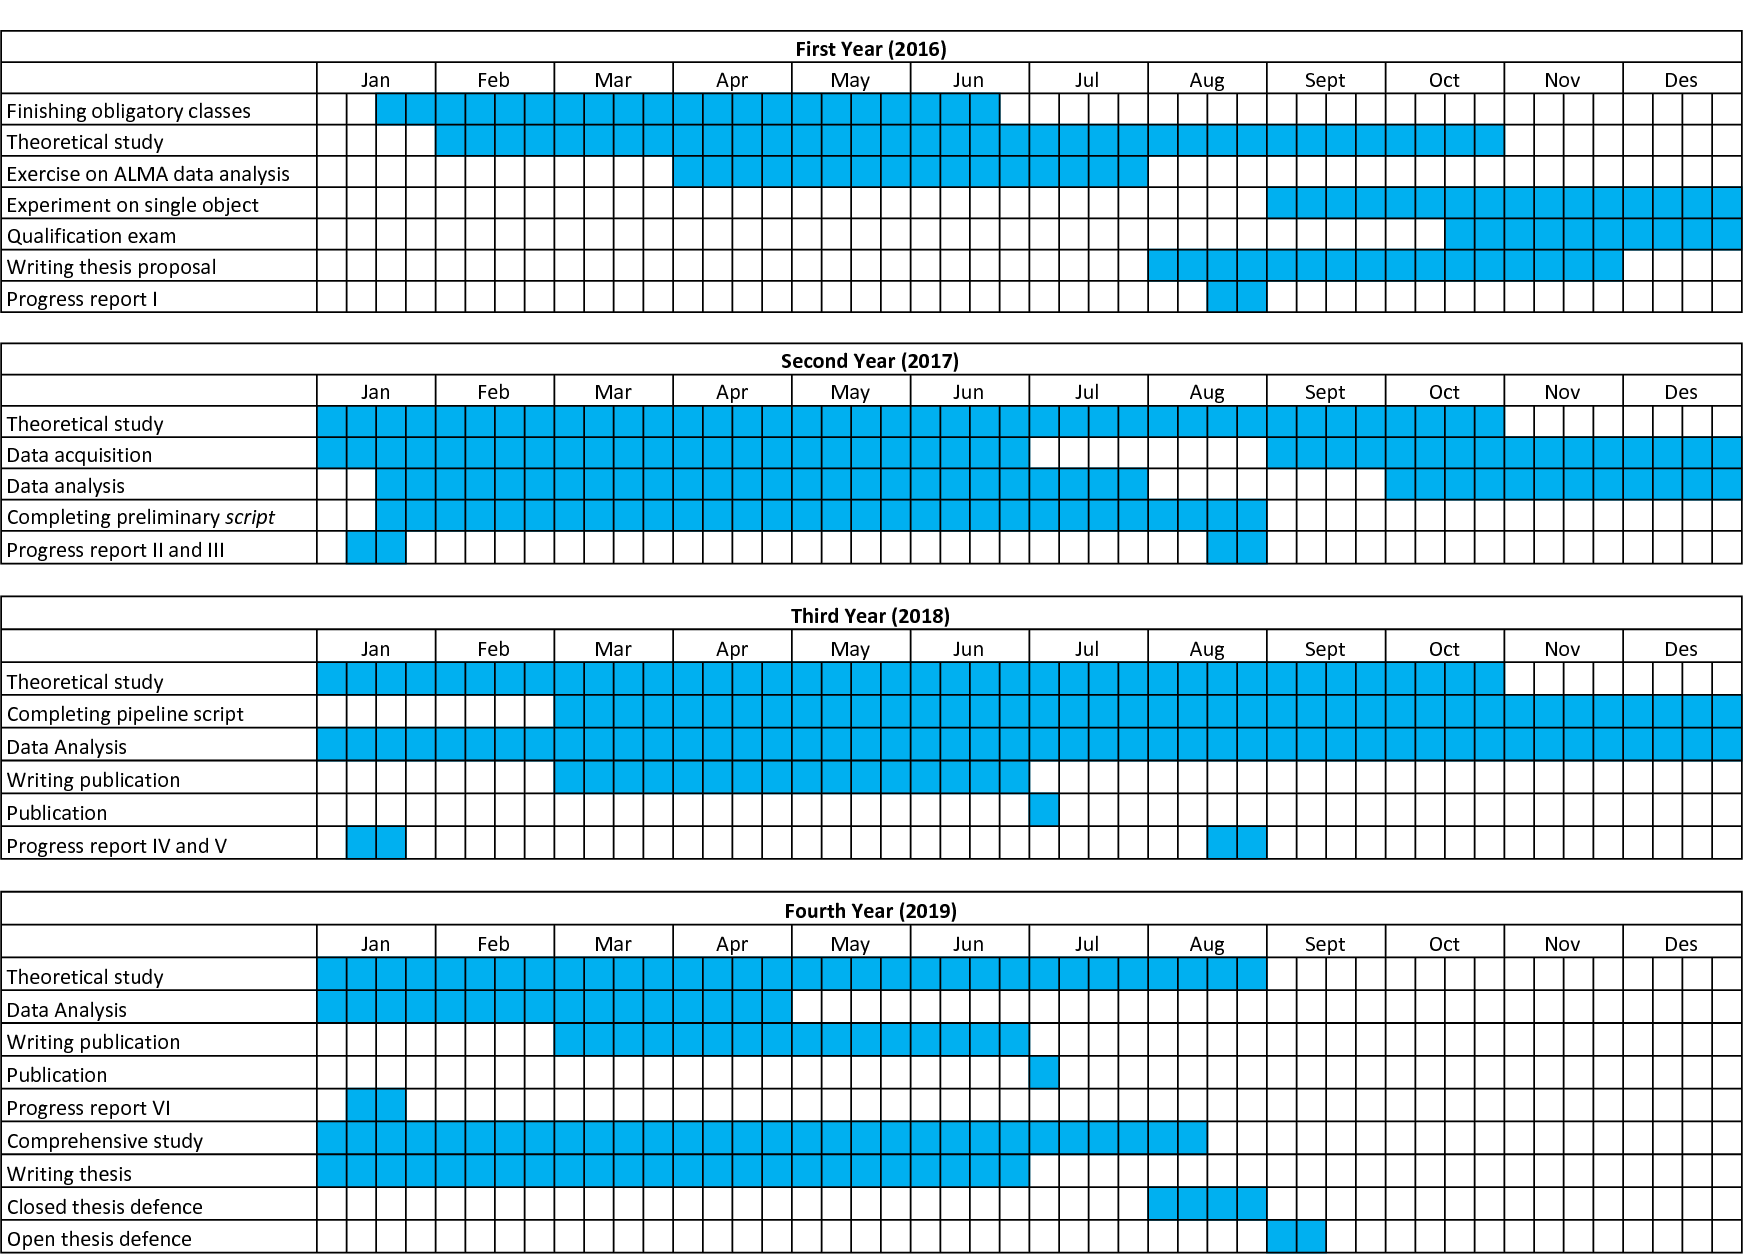
\includegraphics[scale=0.3]{fig/workplan.png}
\caption{Work plan for the first, second, third, and fourth year of doctoral study.}
\label{fig:workplan}
\end{figure}
\end{landscape}

\cleardoublepage

%
\renewcommand\bibname{DAFTAR PUSTAKA}
\bibliography{bibtex}
\addcontentsline{toc}{chapter}{DAFTAR PUSTAKA}
\cleardoublepage
%\appendix 
%\input{biblio.tex}

\end{document}